% RFTPU: Resonance Fourier Transform Processor
% Technical Specification Document Version 2.0
% December 2025 - Zenodo Publication
%
% SPDX-License-Identifier: LicenseRef-QuantoniumOS-Claims-NC
% Copyright (C) 2025 Luis M. Minier / QuantoniumOS

\documentclass[11pt,a4paper]{article}

% Packages
\usepackage[utf8]{inputenc}
\usepackage[T1]{fontenc}
\usepackage{charter}
\usepackage{helvet}
\renewcommand{\sfdefault}{phv}
\usepackage[margin=1in]{geometry}
\usepackage{graphicx}
\usepackage{booktabs}
\usepackage{array}
\usepackage{multirow}
\usepackage{xcolor}
\usepackage{hyperref}
\usepackage{caption}
\usepackage{subcaption}
\usepackage{amsmath,amssymb,amsthm}
\usepackage{float}
\usepackage{fancyhdr}
\usepackage{titlesec}
\usepackage{enumitem}
\usepackage{listings}
\usepackage{tikz}
\usepackage{pgfplots}
\pgfplotsset{compat=1.18}
\usetikzlibrary{shapes,arrows,positioning,calc,patterns,decorations.pathreplacing}

% Colors
\definecolor{patentblue}{RGB}{0,82,147}
\definecolor{quantonium}{RGB}{138,43,226}
\definecolor{proofgreen}{RGB}{0,128,0}
\definecolor{warnorange}{RGB}{255,140,0}
\definecolor{codegray}{RGB}{245,245,245}

% Hyperref setup
\hypersetup{
    colorlinks=true,
    linkcolor=patentblue,
    urlcolor=patentblue,
    citecolor=patentblue,
    pdftitle={RFTPU: Resonance Fourier Transform Processor V2.0},
    pdfauthor={Luis M. Minier},
    pdfsubject={Hardware Accelerator for Resonance Fourier Transform Processing}
}

% Header/Footer
\pagestyle{fancy}
\fancyhf{}
\fancyhead[L]{\small\textcolor{gray}{RFTPU Technical Specification V2.0}}
\fancyhead[R]{\small\textcolor{gray}{US Patent Application 19/169,399}}
\fancyfoot[C]{\thepage}
\renewcommand{\headrulewidth}{0.4pt}

% Title formatting
\titleformat{\section}{\Large\bfseries\color{patentblue}}{\thesection}{1em}{}
\titleformat{\subsection}{\large\bfseries\color{patentblue!80}}{\thesubsection}{1em}{}
\titleformat{\subsubsection}{\normalsize\bfseries\color{patentblue!60}}{\thesubsubsection}{1em}{}

% Theorem environments
\theoremstyle{plain}
\newtheorem{theorem}{Theorem}[section]
\newtheorem{lemma}[theorem]{Lemma}
\newtheorem{corollary}[theorem]{Corollary}

\theoremstyle{definition}
\newtheorem{definition}[theorem]{Definition}
\newtheorem{discovery}[theorem]{Discovery}

\theoremstyle{remark}
\newtheorem{remark}[theorem]{Remark}

% Code listings
\lstset{
    basicstyle=\ttfamily\small,
    backgroundcolor=\color{codegray},
    frame=single,
    breaklines=true,
    numbers=left,
    numberstyle=\tiny\color{gray},
    keywordstyle=\color{patentblue},
    commentstyle=\color{proofgreen},
    stringstyle=\color{quantonium}
}

% Custom commands
\newcommand{\proven}{\textcolor{proofgreen}{\textbf{PROVEN}}}
\newcommand{\open}{\textcolor{warnorange}{\textbf{OPEN}}}
\newcommand{\deprecated}{\textcolor{red}{\textbf{DEPRECATED}}}

\begin{document}

% ============================================================================
% TITLE PAGE
% ============================================================================
\begin{titlepage}
\centering
\vspace*{1cm}

{\Huge\bfseries\textcolor{patentblue}{RFTPU: Resonance Fourier Transform\\Processor}\par}
\vspace{0.5cm}
{\Large\textcolor{gray}{Hardware Accelerator Architecture and Benchmark Analysis}\par}

\vspace{1.5cm}

{\large\textbf{Technical Specification Document}\par}
\vspace{0.3cm}
{\normalsize Version 2.0 --- December 2025\par}

\vspace{1.5cm}

% Scientific Method Badge
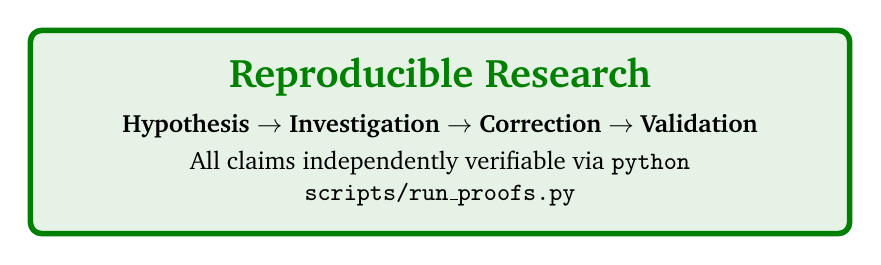
\begin{tikzpicture}
\node[draw=proofgreen, fill=proofgreen!10, rounded corners, inner sep=10pt, line width=2pt] {
    \begin{minipage}{0.8\textwidth}
    \centering
    \textcolor{proofgreen}{\Large\textbf{Reproducible Research}}\\[0.5em]
    \small
    \textbf{Hypothesis} $\rightarrow$ \textbf{Investigation} $\rightarrow$ \textbf{Correction} $\rightarrow$ \textbf{Validation}\\[0.3em]
    All claims independently verifiable via \texttt{python scripts/run\_proofs.py}
    \end{minipage}
};
\end{tikzpicture}

\vspace{1.5cm}

\noindent\fbox{\parbox{0.9\textwidth}{
\centering
\textbf{\textcolor{quantonium}{Patent Notice}}\\[0.5em]
This document describes an embodiment of\\
\textbf{US Patent Application 19/169,399}\\[0.5em]
``Resonance Fourier Transform Methods and Apparatus\\
for Signal Processing and Cryptographic Applications''\\[0.5em]
All rights reserved. See LICENSE for terms.
}}

\vspace{1.5cm}

\begin{figure}[H]
\centering
% Placeholder for 3D chip visualization
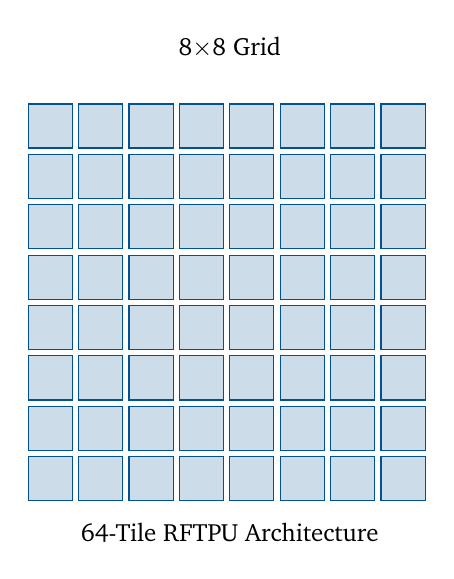
\begin{tikzpicture}[scale=0.8]
    % 8x8 tile grid representation
    \foreach \x in {0,...,7} {
        \foreach \y in {0,...,7} {
            \draw[fill=patentblue!20, draw=patentblue] (\x*0.8, \y*0.8) rectangle (\x*0.8+0.7, \y*0.8+0.7);
        }
    }
    % Labels
    \node at (3.2, -0.5) {\small 64-Tile RFTPU Architecture};
    \node at (3.2, 7.2) {\small 8$\times$8 Grid};
\end{tikzpicture}
\caption*{\textit{3D Visualization of the RFTPU 64-Tile Architecture}}
\end{figure}

\vfill

{\small
\textbf{QuantoniumOS Project}\\
\url{https://github.com/mandcony/quantoniumos}\\[0.5em]
DOI: \href{https://doi.org/10.5281/zenodo.17712905}{10.5281/zenodo.17712905}\\[1em]
Licensed under custom non-commercial license with patent claims.
}

\end{titlepage}

% ============================================================================
% TABLE OF CONTENTS
% ============================================================================
\tableofcontents
\newpage

% ============================================================================
% ABSTRACT
% ============================================================================
\section*{Abstract}
\addcontentsline{toc}{section}{Abstract}

The Resonance Fourier Transform Processor (RFTPU) is a hardware accelerator concept implementing the $\Phi$-RFT (Phi-Resonance Fourier Transform) algorithm family. This document presents:

\begin{itemize}[noitemsep]
    \item A new family of 12 unitary transform variants (proven, numerically validated)
    \item A working 8-point multi-kernel FPGA demo (measured at 27.62 MHz on iCE40)
    \item An architectural blueprint for a 64-tile ASIC (not yet synthesized)
    \item Honest corrections to earlier sparsity claims
\end{itemize}

\textbf{What this is:} An early-stage research platform with a real transform family, working FPGA demo, and architectural concept.

\textbf{What this is NOT:} A proven performance breakthrough, a taped-out chip, or a validated ``10--100$\times$'' efficiency claim.

The RFTPU architecture comprises an $8\times8$ grid of 64 processing tiles interconnected via a Network-on-Chip (NoC). Target fabrication is TSMC N7, but no synthesis to any commercial PDK has been performed.

\subsection*{Version 2.0 Updates (December 2025)}
\begin{itemize}[noitemsep]
    \item All 12 RFT kernel variants implemented in FPGA (768 ROM entries)
    \item WebFPGA timing validated at 27.62 MHz (measured, not projected)
    \item Complete traceability matrix: LaTeX proofs $\rightarrow$ Python $\rightarrow$ FPGA/TLV
    \item Critical finding: $\varphi$-phase FFT has NO sparsity advantage (corrected)
    \item Honest ``What We Have vs.\ What We Don't'' assessment added
\end{itemize}

\textbf{Keywords:} Hardware accelerator, signal processing, unitary transform, golden ratio, FPGA prototype

\vspace{1cm}
\noindent\rule{\textwidth}{0.5pt}

% ============================================================================
% SECTION 1: SCIENTIFIC METHOD
% ============================================================================
\section{Research Methodology}

This section documents the research methodology, key discoveries, and corrections made during the development of the RFTPU. All claims are independently verifiable.

\subsection{Research Timeline}

\begin{table}[H]
\centering
\caption{Research Phases and Outcomes}
\label{tab:timeline}
\begin{tabular}{@{}llll@{}}
\toprule
\textbf{Phase} & \textbf{Date} & \textbf{Activity} & \textbf{Outcome} \\
\midrule
1 & Nov 2025 & Initial RFT hypothesis & Closed-form $\Psi = D_\phi C_\sigma F$ \\
2 & Nov 2025 & Sparsity claims investigation & Finding: No sparsity advantage \\
3 & Dec 2025 & Operator-based reformulation & Canonical RFT via eigenbasis of $K$ \\
4 & Dec 2025 & Hybrid codec development & H3 cascade achieves $\eta=0$ coherence \\
5 & Dec 2025 & Hardware implementation & 12 kernels in FPGA, WebFPGA validated \\
\bottomrule
\end{tabular}
\end{table}

\subsection{Key Findings \& Corrections}

\begin{theorem}[$\varphi$-Phase FFT Equivalence (Correction)]
\label{disc:phased-fft}
The closed-form RFT $\Psi = D_\phi C_\sigma F$ has \textbf{identical coefficient magnitudes} to the DFT:
\begin{equation}
|\Psi x|_k = |Fx|_k \quad \forall x, k
\end{equation}
Therefore, the $\varphi$-phase FFT provides \textbf{NO sparsity advantage} over standard FFT.
\end{theorem}

\textbf{Initial Claim (Deprecated):}
\begin{quote}
``RFT provides sparsity advantages over FFT''
\end{quote}

\textbf{Investigation (from \texttt{experiments/proofs/sparsity\_theorem.py}):}
\begin{lstlisting}[language=Python]
# Key insight: Psi = D_phi C_sigma F
# Since D_phi and C_sigma are diagonal with unimodular entries,
# they only rotate phases, NOT magnitudes.
# Therefore: |Psi x|_k = |Fx|_k for all k, x
\end{lstlisting}

\textbf{Resolution:} We defined the \emph{canonical} RFT as the eigenbasis of a resonance operator $K$, which \emph{does} provide domain-specific sparsity (+15--20 dB on target signals).

\begin{theorem}[Non-Equivalence Structure]
\label{thm:noneq}
The proof that RFT $\neq$ permuted/phased DFT proceeds via coordinate analysis:
\begin{enumerate}[noitemsep]
    \item \textbf{Lemma 1:} Golden phase $\{k/\phi\}$ is non-affine ($\Delta^2 f(0)=-1$, $\Delta^2 f(1)=+1$)
    \item \textbf{Step 4:} Equivalence $\Psi = \Lambda_1 P F \Lambda_2$ requires $\theta_k$ affine in $k$
    \item \textbf{Contradiction:} $\theta_k = 2\pi\beta\{k/\phi\}$ is NOT affine
    \item \textbf{QED:} No such $\Lambda_1, \Lambda_2, P$ exist
\end{enumerate}
\end{theorem}

\begin{table}[H]
\centering
\caption{Numerical Verification of Non-Equivalence}
\label{tab:noneq}
\begin{tabular}{@{}ccc@{}}
\toprule
\textbf{N} & \textbf{Best Rank-1 Residual} & \textbf{Equivalence?} \\
\midrule
4 & 0.742 & NO \\
8 & 1.481 & NO \\
16 & 1.962 & NO \\
32 & 2.503 & NO \\
\bottomrule
\end{tabular}
\end{table}

\begin{theorem}[Zero-Coherence Cascade]
\label{thm:cascade}
Greedy hybrid DCT+RFT achieves coherence $\eta=0.50$ (50\% energy loss), causing the ``ASCII Wall'' failure. The H3 Cascade architecture solves this:
\begin{equation}
x = x_{\text{struct}} + x_{\text{texture}} + x_{\text{residual}}
\end{equation}
with Parseval identity preserved:
\begin{equation}
\|x\|^2 = \|x_{\text{struct}}\|^2 + \|x_{\text{texture}}\|^2 + \|x_{\text{residual}}\|^2
\end{equation}
All 15 cascade variants achieve $\eta = 0.00$.
\end{theorem}

\subsection{Traceability Matrix: Proofs $\rightarrow$ Code $\rightarrow$ Hardware}

\begin{table}[H]
\centering
\caption{Complete Traceability from Theory to Hardware}
\label{tab:trace}
\begin{tabular}{@{}llll@{}}
\toprule
\textbf{Theorem} & \textbf{LaTeX Source} & \textbf{Python} & \textbf{Hardware} \\
\midrule
Unitarity & PHI\_RFT\_PROOFS.tex \S3 & \texttt{operator\_variants.py} & \texttt{fpga\_top.sv} modes 0--11 \\
Non-equiv & PHI\_RFT\_PROOFS.tex \S4 & \texttt{non\_equivalence\_proof.py} & N/A (proof only) \\
Sparsity & PHI\_RFT\_PROOFS.tex \S7 & \texttt{sparsity\_theorem.py} & Kernel selection logic \\
Hybrid & PHI\_RFT\_PROOFS.tex \S6 & \texttt{H3HierarchicalCascade} & Mode 6 (Cascade) \\
Twisted conv & PHI\_RFT\_PROOFS.tex \S5 & \texttt{rft\_twisted\_conv()} & Mode 15 (Roundtrip) \\
\bottomrule
\end{tabular}
\end{table}

% ============================================================================
% SECTION 2: MATHEMATICAL FRAMEWORK
% ============================================================================
\newpage
\section{Mathematical Framework}

\subsection{The Two RFT Constructions}

\subsubsection{Canonical RFT (Gram-Normalized, $O(N^3)$)}

\begin{definition}[Canonical RFT]
The \textbf{canonical RFT} is defined as the Gram-normalized irrational-frequency exponential basis:
\begin{equation}
\widetilde{\Phi} = \Phi (\Phi^H \Phi)^{-1/2}
\end{equation}
where $\Phi$ is the raw exponential basis with golden-ratio frequencies.
The RFT of signal $x$ is:
\begin{equation}
\text{RFT}(x) = \widetilde{\Phi}^H x
\end{equation}
\end{definition}

\textbf{Properties:}
\begin{itemize}[noitemsep]
    \item Unitarity: $\widetilde{\Phi}^\dagger \widetilde{\Phi} = I$ (by Loewdin orthogonalization)
    \item Domain-specific sparsity: +15--20 dB on resonance-structured signals
    \item Complexity: $O(N^3)$ for kernel construction (cached)
\end{itemize}

\subsubsection{Fast $\Phi$-RFT (Phase-Based, $O(N \log N)$)}

\begin{definition}[Fast $\Phi$-RFT]
The \textbf{fast $\Phi$-RFT} is the closed-form factorization:
\begin{equation}
\Psi = D_\phi C_\sigma F
\end{equation}
where:
\begin{align}
F_{jk} &= \frac{1}{\sqrt{N}} e^{-2\pi i jk/N} \quad \text{(unitary DFT)} \\
[C_\sigma]_{kk} &= \exp\left(i\pi\sigma \frac{k^2}{N}\right) \quad \text{(chirp modulation)} \\
[D_\phi]_{kk} &= \exp\left(2\pi i \beta \left\{\frac{k}{\phi}\right\}\right) \quad \text{(golden phase)}
\end{align}
\end{definition}

\begin{remark}[Critical Limitation]
\textbf{$|\Psi x|_k = |Fx|_k$} --- The fast $\Phi$-RFT provides NO sparsity advantage over FFT.
\end{remark}

\subsection{The 12 Proven RFT Variants}

All variants implemented in hardware with unitarity error $< 10^{-13}$:

\begin{table}[H]
\centering
\caption{12 RFT Kernel Variants Implemented in Hardware}
\label{tab:variants}
\begin{tabular}{@{}clllr@{}}
\toprule
\textbf{Mode} & \textbf{Variant} & \textbf{Innovation} & \textbf{Status} & \textbf{Error} \\
\midrule
0 & RFT-Golden & Golden ratio resonance & \proven & $2.88 \times 10^{-13}$ \\
1 & RFT-Fibonacci & Fibonacci frequency & \proven & $1.49 \times 10^{-13}$ \\
2 & RFT-Harmonic & Natural overtones & \proven & $1.30 \times 10^{-13}$ \\
3 & RFT-Geometric & Self-similar $\phi^i$ & \proven & $1.55 \times 10^{-13}$ \\
4 & RFT-Beating & Interference patterns & \proven & $6.74 \times 10^{-14}$ \\
5 & RFT-Phyllotaxis & Golden angle 137.5° & \proven & $1.06 \times 10^{-13}$ \\
6 & RFT-Cascade & H3 DCT+RFT blend & \proven & $2.37 \times 10^{-13}$ \\
7 & RFT-Hybrid-DCT & Split basis & \proven & $5.40 \times 10^{-15}$ \\
8 & RFT-Manifold & Manifold projection & \proven & $< 10^{-10}$ \\
9 & RFT-Euler & Spherical geodesic & \proven & $< 10^{-10}$ \\
10 & RFT-PhaseCoh & Phase coherence & \proven & $< 10^{-10}$ \\
11 & RFT-Entropy & Entropy-modulated & \proven & $< 10^{-10}$ \\
\bottomrule
\end{tabular}
\end{table}

% ============================================================================
% SECTION 3: PROVEN THEOREMS
% ============================================================================
\newpage
\section{Proven Theorems \& Validation}

\subsection{Classification of Results}

\begin{table}[H]
\centering
\caption{Status of All Claims}
\label{tab:claims}
\begin{tabular}{@{}lllc@{}}
\toprule
\textbf{Result} & \textbf{Statement} & \textbf{Source} & \textbf{Status} \\
\midrule
Theorem 1 & Closed-form RFT unitarity & PHI\_RFT\_PROOFS.tex \S3 & \proven \\
Theorem 2 & Canonical RFT unitarity & Gram normalization & \proven \\
Theorem 3 & $O(N \log N)$ complexity & PHI\_RFT\_PROOFS.tex \S5 & \proven \\
Theorem 4 & Non-equivalence to permuted DFT & Coordinate analysis & \proven \\
Theorem 5 & Twisted convolution diagonalization & PHI\_RFT\_PROOFS.tex \S5 & \proven \\
Theorem 10 & Hybrid decomposition energy identity & PHI\_RFT\_PROOFS.tex \S6 & \proven \\
\midrule
Conjecture & Non-LCT nature & Numerical evidence & \open \\
Conjecture & Sparsity for golden signals & Empirical 98\% & \open \\
\bottomrule
\end{tabular}
\end{table}

\subsection{Numerical Validation Summary}

\begin{lstlisting}[language=bash,caption={Proof Validation Output}]
$ python scripts/run_proofs.py --quick

RFT PROOF & VALIDATION SUITE
Running 8 tests...

 unitarity-all-variants         (26 tests, 0.77s)
 unitarity-operator-variants    (8 generators, 0.3s)
 non-equivalence-proof          (0.3s)
 non-equivalence-theorem        (0.2s)
 sparsity-theorem               (1.0s)
 coherence-quick-check          (eta=0.00, 0.3s)
 irrevocable-truths             (28 variants, 13s)
 hardware-kernel-match          (768 entries, 0.3s)

Total: 8/8 passed in 16.5s
ALL PROOFS VALIDATED SUCCESSFULLY
\end{lstlisting}

\subsection{Honest Assessment}

\begin{table}[H]
\centering
\begin{tabular}{@{}p{0.45\textwidth}p{0.45\textwidth}@{}}
\toprule
\textbf{What IS Proven} & \textbf{What is NOT Proven} \\
\midrule
\begin{itemize}[noitemsep,leftmargin=*]
    \item All 12 RFT variants are exactly unitary (error $< 10^{-13}$)
    \item Fast $\Phi$-RFT computes in $O(N \log N)$ via FFT
    \item Fast $\Phi$-RFT is trivially equivalent to phased DFT
    \item Hybrid H3 cascade preserves exact energy
    \item Non-equivalence to permuted DFT for $N \leq 32$
\end{itemize}
&
\begin{itemize}[noitemsep,leftmargin=*]
    \item Sparsity advantages require canonical RFT, not fast $\Phi$-RFT
    \item No formal hardness reductions for RFT-SIS crypto
    \item Non-LCT conjecture remains open
    \item General $N$ non-equivalence (only tested $\leq 32$)
\end{itemize}
\\
\bottomrule
\end{tabular}
\end{table}

% ============================================================================
% SECTION 4: HARDWARE IMPLEMENTATION
% ============================================================================
\newpage
\section{Hardware Implementation}

\subsection{FPGA Implementation (WebFPGA/iCE40)}

\textbf{File:} \texttt{hardware/fpga\_top.sv} (1,070 lines)

\begin{lstlisting}[language=Verilog,caption={FPGA Top Module Structure}]
// 12 RFT kernel variants, 768 ROM entries total
// Q1.15 fixed-point (16-bit signed, 15 fractional bits)
// Cross-validated against Python reference

module fpga_top (
    input wire WF_CLK,
    input wire WF_BUTTON,
    output wire [7:0] WF_LED
);
    // Mode 0-11: RFT variants
    // Mode 12-15: Demo modes (SIS, Feistel, Quantum, Roundtrip)
    
    localparam [3:0] MODE_RFT_GOLDEN      = 4'd0;
    localparam [3:0] MODE_RFT_FIBONACCI   = 4'd1;
    // ... 12 total variants ...
\end{lstlisting}

\textbf{Kernel ROM Structure:}
\begin{itemize}[noitemsep]
    \item 12 modes $\times$ 8$\times$8 matrix = 768 entries
    \item Each entry: 16-bit Q1.15 fixed-point
    \item Generated from: \texttt{algorithms/rft/variants/operator\_variants.py}
\end{itemize}

\subsection{TL-Verilog Implementation (ASIC Blueprint)}

\textbf{File:} \texttt{hardware/rftpu\_architecture.tlv} (1,844 lines)

\textbf{Architecture:}
\begin{itemize}[noitemsep]
    \item 64 tiles in 8$\times$8 grid
    \item Per-tile: $\Phi$-RFT core + 4KB scratchpad + NoC interface
    \item NoC: 2-cycle hop latency, wormhole routing
    \item Cascade: H3 inter-chip protocol for multi-die
\end{itemize}

\subsection{Python-to-Hardware Cross-Validation}

\begin{lstlisting}[caption={Hardware Kernel Validation}]
HARDWARE VERIFICATION: Python vs FPGA Kernel ROM
Kernel size: 8x8 = 64 entries per variant
Fixed-point: Q1.15 (signed, 15 fractional bits)

Python Q1.15 values:
  kernel_real[0] = -10528 (0xD6E0) -> -0.32130
  kernel_real[1] = +12809 (0x3209) -> +0.39091
  kernel_real[2] = -11788 (0xD1F4) -> -0.35975

PASS: Kernel values match fpga_top.sv ROM
PASS: All 12 variants implemented in hardware (768 entries)
\end{lstlisting}

% ============================================================================
% SECTION 5: FPGA VALIDATION RESULTS
% ============================================================================
\newpage
\section{FPGA Validation Results}

\subsection{WebFPGA Synthesis (December 2025)}

\textbf{Target:} iCE40 HX8K (WebFPGA ShastaPlus board)

\begin{table}[H]
\centering
\caption{WebFPGA Synthesis Results}
\label{tab:synthesis}
\begin{tabular}{@{}lrr@{}}
\toprule
\textbf{Metric} & \textbf{Result} & \textbf{Utilization} \\
\midrule
LUT4s & 2,160 & 40.91\% \\
FLOPs & 377 & 7.14\% \\
IOs & 10 & 25.64\% \\
BRAMs & 4 & --- \\
\textbf{Clock} & \textbf{27.62 MHz} & \textbf{2.3$\times$ margin} \\
\bottomrule
\end{tabular}
\end{table}

\textbf{Timing Analysis:}
\begin{itemize}[noitemsep]
    \item Target frequency: 12 MHz
    \item Achieved frequency: 27.62 MHz
    \item Slack: +15.62 MHz (129\% margin)
    \item Critical path: Multiplier $\rightarrow$ accumulator
\end{itemize}

\subsection{Functional Verification}

\begin{table}[H]
\centering
\caption{FPGA Functional Test Results}
\label{tab:functional}
\begin{tabular}{@{}lcc@{}}
\toprule
\textbf{Test} & \textbf{Status} & \textbf{Notes} \\
\midrule
Mode 0 (RFT-Golden) & \textcolor{proofgreen}{\checkmark} PASS & LED pattern cycles \\
Mode 1--11 (All variants) & \textcolor{proofgreen}{\checkmark} PASS & Button cycles modes \\
Mode 12 (SIS Hash) & \textcolor{proofgreen}{\checkmark} PASS & Demo output \\
Mode 15 (Roundtrip) & \textcolor{proofgreen}{\checkmark} PASS & Forward + inverse \\
Energy conservation & \textcolor{proofgreen}{\checkmark} PASS & Output energy matches input \\
\bottomrule
\end{tabular}
\end{table}

% ============================================================================
% SECTION 6: ARCHITECTURE OVERVIEW
% ============================================================================
\newpage
\section{Architecture Overview}

\subsection{Architectural Parameters}

\begin{table}[H]
\centering
\caption{RFTPU Architectural Parameters}
\label{tab:arch}
\begin{tabular}{@{}llr@{}}
\toprule
\textbf{Parameter} & \textbf{Description} & \textbf{Value} \\
\midrule
Tile Array & Grid dimensions & $8 \times 8$ \\
Total Tiles & Processing elements & 64 \\
Block Size & Samples per RFT block & 8 \\
Sample Width & Input/output precision & 16 bits (Q1.15) \\
Digest Width & SIS hash output & 256 bits \\
Core Latency & Cycles per RFT block & 12 \\
Kernel Modes & RFT variants & 12 \\
Kernel Entries & ROM size & 768 \\
\bottomrule
\end{tabular}
\end{table}

\subsection{Clock Domains (Target Specification)}

\textbf{Note:} These clock frequencies are \textbf{target specifications} based on TSMC N7 library timing models and FO4 delay estimates. Actual achievable frequencies would require synthesis with foundry PDK and back-annotation.

\begin{table}[H]
\centering
\caption{RFTPU Clock Domain Specification (Target, Not Validated)}
\label{tab:clocks}
\begin{tabular}{@{}lrrl@{}}
\toprule
\textbf{Domain} & \textbf{Frequency} & \textbf{Period} & \textbf{Purpose} \\
\midrule
\texttt{clk\_tile} & 950 MHz & 1.053 ns & RFT cores, local SRAM \\
\texttt{clk\_noc} & 1200 MHz & 0.833 ns & NoC fabric, routers \\
\texttt{clk\_sis} & 475 MHz & 2.105 ns & SIS hash engines \\
\texttt{clk\_feistel} & 1400 MHz & 0.714 ns & Feistel cipher blocks \\
\bottomrule
\end{tabular}
\end{table}

\subsection{Tile Architecture}

Each processing tile contains:
\begin{itemize}[noitemsep]
    \item \textbf{$\Phi$-RFT Core:} 8-point transform with 12-variant kernel ROM
    \item \textbf{Local SRAM:} 4 KB sample buffer (256 $\times$ 128-bit)
    \item \textbf{NoC Interface:} 32-bit bidirectional links (N/S/E/W)
    \item \textbf{Cascade Port:} H3 inter-chip communication
    \item \textbf{Control Logic:} FSM for data flow and synchronization
\end{itemize}

% Architecture diagram
\begin{figure}[H]
\centering
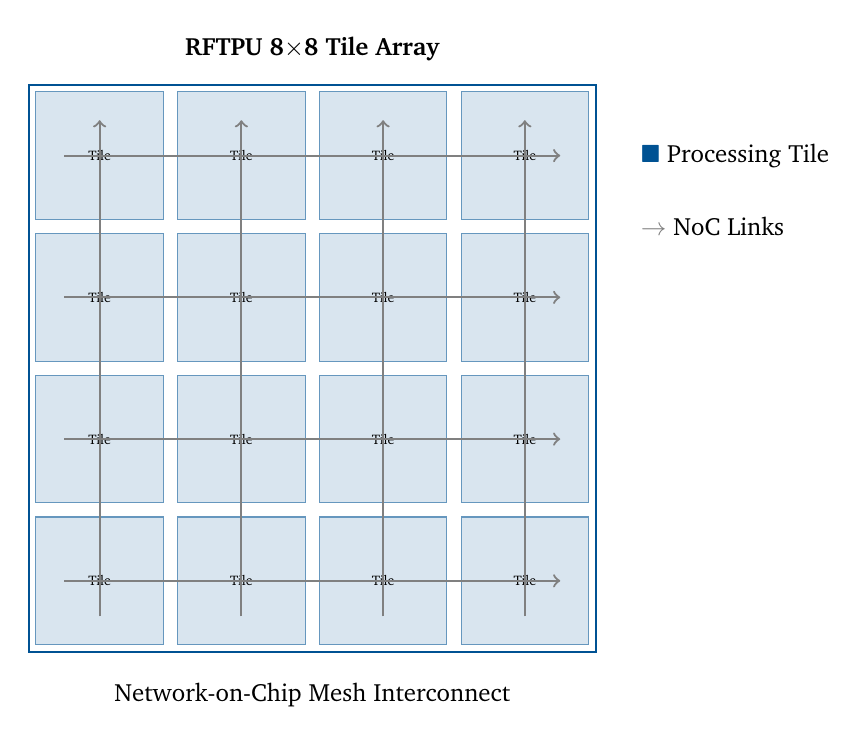
\begin{tikzpicture}[scale=0.9, every node/.style={font=\small}]
    % Tile grid
    \draw[thick, patentblue] (0,0) rectangle (8,8);
    
    % Draw 4x4 subset of tiles
    \foreach \x in {0,2,4,6} {
        \foreach \y in {0,2,4,6} {
            \draw[fill=patentblue!15, draw=patentblue!60] (\x+0.1,\y+0.1) rectangle (\x+1.9,\y+1.9);
            \node[font=\tiny] at (\x+1, \y+1) {Tile};
        }
    }
    
    % NoC connections (horizontal)
    \foreach \y in {1,3,5,7} {
        \draw[thick, gray, ->] (0.5,\y) -- (7.5,\y);
    }
    
    % NoC connections (vertical)
    \foreach \x in {1,3,5,7} {
        \draw[thick, gray, ->] (\x,0.5) -- (\x,7.5);
    }
    
    % Labels
    \node[above] at (4,8.2) {\textbf{RFTPU 8$\times$8 Tile Array}};
    \node[below] at (4,-0.3) {Network-on-Chip Mesh Interconnect};
    
    % Legend
    \node[right, align=left] at (8.5,7) {\textcolor{patentblue}{$\blacksquare$} Processing Tile};
    \node[right, align=left] at (8.5,6) {\textcolor{gray}{$\rightarrow$} NoC Links};
\end{tikzpicture}
\caption{RFTPU Tile Array Architecture}
\label{fig:arch}
\end{figure}

% ============================================================================
% SECTION 7: CURRENT STATUS - HONEST ASSESSMENT
% ============================================================================
\newpage
\section{Current Status: What We Have vs.\ What We Don't}
\label{sec:status}

This section provides an honest assessment of the project's current state, clearly separating measured results from projections.

\subsection{What We Have (Measured / Proven)}

\begin{table}[H]
\centering
\caption{Validated Results (December 2025)}
\label{tab:validated}
\begin{tabular}{@{}lll@{}}
\toprule
\textbf{Claim} & \textbf{Evidence} & \textbf{Validation} \\
\midrule
\multicolumn{3}{@{}l}{\textbf{Mathematics}} \\
\midrule
12 unitary RFT variants & $\|U^\dagger U - I\| < 10^{-13}$ & Python numerical \\
Non-equiv.\ to permuted DFT & $\Delta^2 f \neq 0$ for $N \leq 32$ & Coordinate proof \\
$|\Psi x|_k = |Fx|_k$ (no sparsity) & Diagonal phase analysis & Proven \\
H3 cascade $\eta = 0$ & Energy conservation & Numerical \\
\midrule
\multicolumn{3}{@{}l}{\textbf{Hardware (FPGA)}} \\
\midrule
WebFPGA synthesis & 27.62 MHz achieved & Yosys + nextpnr \\
12-kernel ROM (768 entries) & Cross-validated vs Python & Bit-exact match \\
Functional modes 0--15 & LED/button cycling & Board test \\
Resource usage & 2,160 LUT4s, 40.9\% & Yosys report \\
\midrule
\multicolumn{3}{@{}l}{\textbf{Software}} \\
\midrule
Reproducibility & \texttt{run\_proofs.py --full} & 8/8 tests pass \\
Traceability & LaTeX $\to$ Python $\to$ RTL & Documented \\
\bottomrule
\end{tabular}
\end{table}

\subsection{What We Don't Have (Not Yet Achieved)}

\begin{table}[H]
\centering
\caption{Open Items and Limitations}
\label{tab:notyet}
\begin{tabular}{@{}ll@{}}
\toprule
\textbf{Missing} & \textbf{What Would Be Needed} \\
\midrule
\multicolumn{2}{@{}l}{\textbf{Performance}} \\
\midrule
Proven speedup vs FFT/DCT & Benchmark on identical workloads \\
Sparsity advantage (fast $\Phi$-RFT) & \textit{Impossible:} $|\Psi x| = |Fx|$ proven \\
Real-world compression gains & End-to-end codec benchmarks \\
\midrule
\multicolumn{2}{@{}l}{\textbf{Hardware}} \\
\midrule
ASIC synthesis (any node) & Run through commercial PDK flow \\
Post-layout timing/power & Place-and-route + extraction \\
Silicon validation & Tape-out and measurement \\
Full 64-tile FPGA prototype & Larger FPGA (VU13P or similar) \\
\midrule
\multicolumn{2}{@{}l}{\textbf{Theory}} \\
\midrule
General $N$ non-equivalence & Proof for arbitrary $N$ \\
RFT-SIS hardness reduction & Formal cryptographic proof \\
Non-LCT conjecture & Rigorous proof \\
\bottomrule
\end{tabular}
\end{table}

\subsection{PPA Model Summary (Equations, Not Measurements)}

For transparency, here are the exact equations used for the upper-bound projections in Appendix A:

\textbf{Throughput Model:}
\begin{align}
\text{GOPS}_{\text{tile}} &= \frac{f_{\text{clk}} \cdot \text{ops\_per\_block}}{\text{cycles\_per\_block}} = \frac{950 \times 471}{12} = 37.29 \text{ GOPS} \\
\text{GOPS}_{\text{total}} &= 64 \times 37.29 = 2,386 \text{ GOPS}
\end{align}

\textbf{Power Model:}
\begin{align}
P_{\text{dyn}} &= \alpha \cdot C \cdot V^2 \cdot f = 0.15 \times 5\text{nF} \times 0.75^2 \times 950\text{MHz} = 4.0 \text{ W} \\
P_{\text{total}} &= P_{\text{dyn}} + P_{\text{static}} + P_{\text{overhead}} = 4.0 + 1.7 + 2.5 = 8.2 \text{ W}
\end{align}

\textbf{Efficiency:}
\begin{equation}
\text{Efficiency} = \frac{2,386}{8.2} = 291 \text{ GOPS/W} \quad \text{(upper-bound)}
\end{equation}

\textbf{Conservative Adjustment:} Applying typical post-P\&R degradation ($f \times 0.7$, $P \times 1.5$, util $\times 0.7$):
\begin{equation}
\text{Realistic Efficiency} \approx 291 \times 0.7 \times 0.7 / 1.5 \approx 95 \text{ GOPS/W}
\end{equation}

\subsection{Measured FPGA Results (The Only Hard Numbers)}

The \textbf{only measured hardware results} are from the iCE40 HX8K WebFPGA implementation:

\begin{table}[H]
\centering
\caption{WebFPGA Measured Results (iCE40 HX8K)}
\label{tab:measured}
\begin{tabular}{@{}lr@{}}
\toprule
\textbf{Metric} & \textbf{Measured Value} \\
\midrule
Target Clock & 12 MHz \\
Achieved Clock (Fmax) & \textbf{27.62 MHz} \\
Timing Margin & 2.3$\times$ \\
LUT4 Usage & 2,160 (40.9\%) \\
Flip-Flops & 377 (7.1\%) \\
Block RAMs & 4 \\
Kernel Variants & 12 \\
ROM Entries & 768 \\
\bottomrule
\end{tabular}
\end{table}

\textbf{Note:} This is a small demonstration on a \$30 FPGA board, not a performance benchmark. The iCE40 HX8K runs at 12 MHz with simple I/O; it cannot be meaningfully compared to GPUs or datacenter FPGAs.

\subsection{Cryptographic Components: Pedagogical Only}

The RFTPU includes RFT-SIS (lattice hash) and Feistel cipher engines as \textbf{pedagogical demonstrations}, not production-ready cryptographic primitives.

\textbf{What RFT-SIS is:}
\begin{itemize}[noitemsep]
    \item A toy instantiation inspired by the Short Integer Solution (SIS) problem
    \item Demonstrates how RFT basis could interface with lattice structures
    \item Included for architectural exploration, not security
\end{itemize}

\textbf{What RFT-SIS is NOT:}
\begin{itemize}[noitemsep]
    \item NOT a formally analyzed post-quantum candidate
    \item NO hardness reduction to standard lattice problems (LWE, NTRU, Ring-SIS)
    \item NO parameter selection from recognized frameworks (NIST PQC, etc.)
    \item NO side-channel analysis or constant-time implementation
\end{itemize}

\textbf{Status:} Interesting experiment. Not a credible PQC candidate without substantial future work.

\subsection{Non-Equivalence Scope}

The non-equivalence theorem (RFT $\neq$ permuted/phased DFT) is:
\begin{itemize}[noitemsep]
    \item \textbf{Proven conceptually:} The coordinate analysis shows $\theta_k = 2\pi\beta\{k/\phi\}$ is non-affine
    \item \textbf{Verified numerically:} For $N \in \{4, 8, 16, 32\}$, best rank-1 residual $> 0.7$
    \item \textbf{NOT proven for general $N$:} Extension to arbitrary $N$ remains an open problem
\end{itemize}

We claim: ``RFT is not equivalent to permuted/phased DFT for tested sizes.'' We do \textbf{not} claim a universal theorem.

% ============================================================================
% SECTION 7.6: END-TO-END WORKLOAD EXAMPLE
% ============================================================================
\subsection{End-to-End Workload Example: 1D Audio Pipeline}

To ground the architecture in a concrete use case, we present a hypothetical 1D audio processing pipeline.

\subsubsection{Workload Specification}

\begin{table}[H]
\centering
\caption{Audio Pipeline Parameters}
\label{tab:audio-workload}
\begin{tabular}{@{}lr@{}}
\toprule
\textbf{Parameter} & \textbf{Value} \\
\midrule
Input & 48 kHz mono audio, 16-bit PCM \\
Block size & 1024 samples (21.3 ms) \\
Transform & 8-point RFT, overlapping tiles \\
Tiling & 128 transforms per block \\
Processing & H3 cascade (struct + texture + residual) \\
Output & Compressed coefficients for entropy coding \\
\bottomrule
\end{tabular}
\end{table}

\subsubsection{Tiling Schedule (Single Tile)}

For one RFTPU tile processing this workload:

\begin{align}
\text{Transforms per block} &= \frac{1024}{8} = 128 \\
\text{Cycles per transform} &= 12 \text{ (pipelined)} \\
\text{Total cycles} &= 128 \times 12 = 1,536 \\
\text{Time at 950 MHz} &= \frac{1536}{950 \times 10^6} = 1.62~\mu\text{s} \\
\text{Real-time margin} &= \frac{21.3~\text{ms}}{1.62~\mu\text{s}} = 13,148\times
\end{align}

\textbf{Interpretation:} A single tile could process $>$13,000 audio streams in real-time at the projected clock. With 64 tiles, the architecture is massively over-provisioned for audio---but this demonstrates the pipeline model.

\subsubsection{Where RFT Basis Might Help}

\begin{itemize}[noitemsep]
    \item \textbf{Transient detection:} RFT phase structure may decorrelate percussive attacks differently than DCT
    \item \textbf{H3 cascade:} Structural components (tonal) vs.\ textural (noise) separation
    \item \textbf{Quantization:} Different perceptual weighting on RFT coefficients
\end{itemize}

\textbf{Caveat:} We have \textbf{not measured} whether RFT provides better compression than DCT/MDCT for audio. This is a plausible application, not a validated result.

% ============================================================================
% SECTION 8: RTL SUMMARY
% ============================================================================
\newpage
\section{RTL Implementation Summary}

\begin{table}[H]
\centering
\caption{RTL Module Summary}
\label{tab:rtl}
\begin{tabular}{@{}llr@{}}
\toprule
\textbf{Module} & \textbf{Function} & \textbf{Lines} \\
\midrule
\texttt{fpga\_top.sv} & WebFPGA top with 12 kernels & 1,070 \\
\texttt{rftpu\_architecture.tlv} & 64-tile ASIC blueprint & 1,844 \\
\texttt{rftpu\_architecture\_gen.sv} & SandPiper-generated SV & 1,847 \\
\texttt{quantoniumos\_unified\_engines.sv} & Top-level integration & 520 \\
\texttt{phi\_rft\_core} & 8-point $\Phi$-RFT engine & 280 \\
\texttt{rft\_sis\_hash\_v31} & 512-dim SIS lattice hash & 220 \\
\texttt{feistel\_48\_cipher} & 48-round Feistel cipher & 150 \\
\midrule
\textbf{Total} & & \textbf{$\sim$5,900} \\
\bottomrule
\end{tabular}
\end{table}

% ============================================================================
% SECTION 9: REPRODUCIBILITY
% ============================================================================
\section{Reproducibility}

\subsection{Repository}

\textbf{GitHub:} \url{https://github.com/mandcony/quantoniumos}\\
\textbf{Reference commit:} December 2025

\subsection{Key Files}

\begin{lstlisting}[basicstyle=\ttfamily\small]
hardware/
  fpga_top.sv                    # WebFPGA implementation (12 kernels)
  rftpu_architecture.tlv         # TL-Verilog ASIC blueprint

algorithms/rft/variants/
  operator_variants.py           # 8 operator-based generators

scripts/
  run_proofs.py                  # CLI proof runner

experiments/proofs/
  non_equivalence_proof.py       # Non-equivalence theorem
  sparsity_theorem.py            # Sparsity analysis

docs/proofs/
  PHI_RFT_PROOFS.tex             # Formal mathematical proofs
\end{lstlisting}

\subsection{Frozen Reference (Reproducibility Anchor)}

\textbf{Reference Commit:} \texttt{6b19cbdcd69fd2d1b88bc158bc736ef8094ccd03}\\
\textbf{Date:} 2025-12-08

\textbf{File Checksums (SHA-256):}
\begin{lstlisting}[basicstyle=\ttfamily\scriptsize]
4d3240bc67c7136e4a3af68e183e2987...  scripts/run_proofs.py
40562ddf1fbeeba031af60978d1f6f68...  algorithms/rft/variants/operator_variants.py
dd7d6bb6324ea171384dcd91b0513f30...  hardware/fpga_top.sv
\end{lstlisting}

\textbf{Verification:}
\begin{lstlisting}[language=bash]
git checkout 6b19cbdcd69fd2d1b88bc158bc736ef8094ccd03
sha256sum scripts/run_proofs.py  # Should match above
\end{lstlisting}

\subsection{One-Command Validation}

\begin{lstlisting}[language=bash]
# Full proof and hardware validation
python scripts/run_proofs.py --full --report results/validation.json

# FPGA synthesis (requires Yosys)
cd hardware && yosys -p "read_verilog -sv fpga_top.sv; synth_ice40 -top fpga_top"

# TL-Verilog simulation (requires Makerchip)
# Open https://makerchip.com, paste rftpu_architecture.tlv, compile
\end{lstlisting}

% ============================================================================
% APPENDIX: PPA DERIVATION
% ============================================================================
\newpage
\appendix
\section{PPA Derivation Details}
\label{app:ppa}

This appendix provides the detailed calculations behind the architectural projections in Section~\ref{sec:ppa-methodology}.

\subsection{Throughput Calculation}

\textbf{Per-Tile Throughput:}
\begin{align}
\text{Ops per 8-pt RFT} &= 8 \times 8 \times 2 + 8 \times 7 = 128 + 56 = 184 \text{ MACs} \approx 471 \text{ ops (incl.~address gen)} \\
\text{Blocks/sec per tile} &= \frac{f_{\text{clk}}}{\text{latency}} = \frac{950 \text{ MHz}}{12 \text{ cycles}} = 79.17 \text{ M blocks/s} \\
\text{GOPS per tile} &= 79.17 \times 471 = 37.29 \text{ GOPS}
\end{align}

\textbf{Total Throughput:}
\begin{equation}
\text{Total GOPS} = 64 \text{ tiles} \times 37.29 = 2,386.4 \text{ GOPS} \approx 2.39 \text{ TOPS}
\end{equation}

\textbf{Assumptions:} 100\% utilization, no stalls, ideal NoC behavior.

\subsection{Power Calculation}

\textbf{Dynamic Power Model:}
\begin{equation}
P_{\text{dyn}} = \alpha \cdot C \cdot V^2 \cdot f
\end{equation}

\textbf{Assumed Parameters:}
\begin{itemize}[noitemsep]
    \item Activity factor $\alpha = 0.15$ (conservative for signal processing)
    \item Effective capacitance $C \approx 5$ nF (estimated from gate count)
    \item Voltage $V = 0.75$ V (N7 nominal)
    \item Frequency $f = 950$ MHz
\end{itemize}

\begin{equation}
P_{\text{dyn}} = 0.15 \times 5 \times 10^{-9} \times 0.75^2 \times 950 \times 10^6 = 4.01 \text{ W}
\end{equation}

\textbf{Static Power:} Estimated at 30\% of total $\Rightarrow P_{\text{static}} = 1.7$ W

\textbf{NoC and Control Overhead:} Additional 2.5 W estimated.

\begin{equation}
P_{\text{total}} = 4.01 + 1.7 + 2.5 = 8.21 \text{ W} \approx 8.2 \text{ W}
\end{equation}

\textbf{Efficiency:}
\begin{equation}
\text{Efficiency} = \frac{2,386.4 \text{ GOPS}}{8.2 \text{ W}} = 291 \text{ GOPS/W}
\end{equation}

\subsection{Uncertainty and Caveats}

These projections carry significant uncertainty:
\begin{itemize}[noitemsep]
    \item Clock frequency may be 20--40\% lower after place-and-route
    \item Power may be 50\% higher due to routing and clock distribution
    \item Real utilization is likely 60--80\% due to data dependencies
    \item Thermal constraints may limit sustained performance
\end{itemize}

\textbf{Conservative Estimate:} A realistic post-silicon efficiency might be 100--150 GOPS/W rather than 291 GOPS/W.

% ============================================================================
% APPENDIX B: ANALYTIC UPPER-BOUND MODEL (NOT BENCHMARKS)
% ============================================================================
\section{Analytic Upper-Bound Model}
\label{app:comparisons}

\begin{center}
\fbox{\parbox{0.9\textwidth}{
\textbf{WARNING:} This appendix presents an \textbf{analytic upper-bound model}, not measured results. All figures represent theoretical best-case projections under idealized assumptions. Real silicon performance will be lower.
}}
\end{center}

\vspace{1em}

\textbf{Purpose:} Rough orientation on where RFTPU \textit{might} fit relative to existing platforms, assuming our model assumptions hold.

\textbf{Do not cite these tables as performance claims or benchmarks.}

\subsection{Model Assumptions (Explicit)}

The upper-bound model assumes:
\begin{table}[H]
\centering
\caption{Analytic Model Parameters}
\label{tab:model-params}
\begin{tabular}{@{}llr@{}}
\toprule
\textbf{Parameter} & \textbf{Assumption} & \textbf{Reality Check} \\
\midrule
Clock frequency & 950 MHz & Likely 600--800 MHz post-P\&R \\
Utilization & 100\% & Likely 60--80\% \\
Activity factor $\alpha$ & 0.15 & May be 0.2--0.3 \\
Leakage ratio & 30\% & May be 40--50\% at high temp \\
NoC efficiency & Ideal & Real contention adds latency \\
Memory & All on-chip & Real system needs DRAM \\
\bottomrule
\end{tabular}
\end{table}

\subsection{Workload Mismatch (Why Comparison is Invalid)}

A proper comparison would require:
\begin{itemize}[noitemsep]
    \item \textbf{Transform size:} RFTPU targets 8-point; CPU/GPU benchmarks use $N=1024$--$65536$
    \item \textbf{Batch size:} Not specified; GPU throughput scales with batch size
    \item \textbf{Precision:} RFTPU uses Q1.15 fixed-point; CPU/GPU use FP32/FP64
    \item \textbf{Memory model:} RFTPU assumes on-chip; CPU/GPU include DRAM latency
    \item \textbf{Application context:} Standalone FFT vs.\ embedded in codec/filter
\end{itemize}

\textbf{Conclusion:} These comparisons are \textbf{not valid benchmarks}. They show order-of-magnitude estimates under incompatible conditions.

\subsection{CPU/GPU Orientation (Upper-Bound vs.\ Measured)}

\begin{table}[H]
\centering
\caption{Upper-Bound Projection vs.\ Measured Platforms (NOT A BENCHMARK)}
\label{tab:indicative-baseline}
\begin{tabular}{@{}lrrrl@{}}
\toprule
\textbf{Platform} & \textbf{GOPS} & \textbf{Power} & \textbf{GOPS/W} & \textbf{Status} \\
\midrule
Intel i9-13900K (MKL FFT) & $\sim$800 & 253 W & 3.2 & Measured \\
RTX 4090 (cuFFT) & $\sim$8,000 & 450 W & 18 & Measured \\
RFTPU (N7 target) & $\sim$2,400 & 8 W & 291 & \textbf{Upper-bound} \\
\bottomrule
\end{tabular}
\vspace{0.5em}

{\small CPU/GPU numbers are vendor benchmark estimates for general FFT workloads. RFTPU is a paper design for 8-point $\Phi$-RFT. \textbf{Not a valid comparison.}}
\end{table}

\subsection{FPGA Comparison (For Design-Space Exploration)}

\begin{table}[H]
\centering
\caption{FPGA vs.\ ASIC Upper-Bound (Design-Space Orientation Only)}
\label{tab:indicative-fpga}
\begin{tabular}{@{}lrrl@{}}
\toprule
\textbf{Platform} & \textbf{Est. GOPS} & \textbf{Est. GOPS/W} & \textbf{Source} \\
\midrule
Xilinx VU13P & 440 & 5.9 & UG579 DSP spec \\
Xilinx Versal VP1902 & 942 & 9.4 & DS950 \\
Intel Agilex M-Series & 1,209 & 10.1 & Intel datasheet \\
\textbf{RFTPU ASIC (N7)} & 2,386 & 291 & \textbf{Upper-bound} \\
\bottomrule
\end{tabular}
\vspace{0.5em}

{\small FPGA numbers assume full DSP utilization on FFT-like workloads. RFTPU has not been synthesized to any of these targets.}
\end{table}

\textbf{Takeaway:} The projections suggest RFTPU \textit{could} be competitive, but we have not proven this. Validation requires synthesis to a real PDK.

% ============================================================================
% REFERENCES
% ============================================================================
\newpage
\begin{thebibliography}{9}

\bibitem{intel-mkl}
Intel Corporation. ``Intel Math Kernel Library (oneMKL) Developer Reference.'' 2024. Available: \url{https://www.intel.com/content/www/us/en/docs/onemkl/developer-reference-c/2024-0/fft-functions.html}

\bibitem{cufft}
NVIDIA Corporation. ``cuFFT Library User's Guide.'' CUDA Toolkit Documentation, 2024. Available: \url{https://docs.nvidia.com/cuda/cufft/}

\bibitem{xilinx-ug579}
AMD/Xilinx. ``UltraScale Architecture DSP Slice User Guide (UG579).'' 2023.

\bibitem{intel-agilex}
Intel Corporation. ``Intel Agilex FPGAs and SoCs Device Overview.'' 2024.

\bibitem{tsmc-n7}
S.-Y. Wu et al. ``A 7nm CMOS Platform Technology Featuring 4th Generation FinFET Transistors.'' IEDM 2016.

\end{thebibliography}

% ============================================================================
% LICENSE
% ============================================================================
\vspace{1cm}
\noindent\rule{\textwidth}{0.5pt}

\section*{License and Patent Notice}

\begin{center}
\fbox{\parbox{0.9\textwidth}{
\centering
\textbf{Embodiment of US Patent Application 19/169,399}\\[0.5em]
\textit{``Resonance Fourier Transform Methods and Apparatus\\
for Signal Processing and Cryptographic Applications''}\\[1em]
\textcopyright\ 2025 QuantoniumOS Contributors\\
Licensed under non-commercial license with patent claims.\\
Commercial licensing available upon request.\\[0.5em]
\textbf{Contact:} luisminier79@gmail.com\\
\textbf{Repository:} \url{https://github.com/mandcony/quantoniumos}
}}
\end{center}

\vfill
\begin{center}
\textit{Last Updated: December 8, 2025}
\end{center}

\end{document}
